\appchapter[RL Agent Training]{RL Agent Training}
\label{appendix:d}

% Phase 1
% We observe that the RL agent converges to 10 interactive threads and 10 batch threads. The results are showing in figure X.

% Phase 2
% We observe that the RL agent converges to 10 interactive threads and 10 batch threads. The results are showing in figure X.

% Phase 3
% We observe that the RL agent converges to 10 interactive threads and 10 batch threads. The results are showing in figure X.

% Phase 4
% We observe that the RL agent converges to 10 interactive threads and 10 batch threads. The results are showing in figure X.

\begin{table}[ht]
    \centering
    \caption{Model Selection and Hyper-parameter Tuning}
    \label{table:hyperparameter_tuning}
    % Tabular environment goes AFTER the caption!
    % \begin{adjustbox}{width=1\textwidth}
    \begin{tabular}{|c|c|c|}
      % after \\: \hline or \cline{col1-col2} \cline{col3-col4} ...
      \hline
      \thead{Type} & \thead{Parameter} & \thead{Values} \\
      \hline
      Preprocessing & Degree & 1,2,3 \\\hline
      Regression & alpha & 0.1, 0.01, 0.001, 0.0001 \\\hline
      Regression & penalty & l1, l2, elasticnet \\\hline
      Regression & loss & squared, huber, epsilon\_insensitive \\\hline
      Regression & learning rate & constant, optimal, invscaling \\\hline
      Regression & max\_iterations & 100, 1000, 10000, 100000 \\
      \hline
    \end{tabular}
  % \end{adjustbox}
  \end{table}
  
  \begin{table}[ht]
    \centering
    \caption{Resulting Linear Regression Models}
    \label{table:per_model_parameters}
    % Tabular environment goes AFTER the caption!
    \begin{adjustbox}{width=1\textwidth}
    \begin{tabular}{|c|c|c|}
      % after \\: \hline or \cline{col1-col2} \cline{col3-col4} ...
      \hline
      \thead{Model} & \thead{Action} & \thead{Parameters} \\
      \hline
      Model\_1 & 1 & learning\_rate: invscaling, loss: squared\_loss, alpha: 0.001, max\_iter: 10000, penalty: l2 \\\hline
      Model\_2 & 2 & learning\_rate: invscaling, loss: squared\_loss, alpha: 0.0001, max\_iter: 1000, penalty: l2 \\\hline
      Model\_3 & 3 & learning\_rate: invscaling, loss: squared\_loss, alpha: 0.001, max\_iter: 1000, penalty: elasticnet \\\hline
      Model\_4 & 4 & learning\_rate: invscaling, loss: squared\_loss, alpha: 0.0001, max\_iter: 10000, penalty: l1 \\\hline
      Model\_5 & 5 & learning\_rate: invscaling, loss: squared\_loss, alpha: 0.01, max\_iter: 100, penalty: elasticnet \\\hline
      Model\_6 & 6 & learning\_rate: invscaling, loss: squared\_loss, alpha:  0.001, max\_iter: 10000, penalty: l2 \\\hline
      Model\_7 & 7 & learning\_rate: invscaling, loss: squared\_loss, alpha: 0.01, max\_iter: 1000, penalty: elasticnet \\\hline
      Model\_8 & 8 & learning\_rate: invscaling, loss: squared\_loss, alpha: 0.001, max\_iter: 100, penalty: l1 \\\hline
      Model\_9 & 9 & learning\_rate: invscaling, loss: squared\_loss, alpha: 0.0001, max\_iter: 100, penalty: elasticnet \\
      \hline
    \end{tabular}
  \end{adjustbox}
  \end{table}
  
  \begin{table}[ht]
    \centering
    \caption{Q-Learning Parameters}
    \label{table:rl_training_parameters}
    % Tabular environment goes AFTER the caption!
    % \begin{adjustbox}{width=1\textwidth}
    \begin{tabular}{|c|c|}
      % after \\: \hline or \cline{col1-col2} \cline{col3-col4} ...
      \hline
      \thead{Parameter} & \thead{Value} \\
      \hline
      episodes & Phases $1-2$: 700, Phases $3-4$: 1,000 \\\hline
      Per-episode steps & 200 \\\hline
      gamma & 0.95 \\\hline
      learning rate & 0.7 \\\hline
      epsilon & 0.9 \\\hline
      epsilon\_decay & 0.1 \\\hline
      Target 99th Latency & $\leq 250 microseconds$ \\\hline
      Target throughput & $\geq 250,000 operations/second$ \\
      \hline
    \end{tabular}
  % \end{adjustbox}
  \end{table}

  \begin{table}[ht]
    \centering
    \caption{Preliminary Rewards Phase 1}
    \label{table:rewards_phase_1}
    % Tabular environment goes AFTER the caption!
    % \begin{adjustbox}{width=1\textwidth}
    \begin{tabular}{|c|c|c|c|c|c|}
      % after \\: \hline or \cline{col1-col2} \cline{col3-col4} ...
      \hline
      \thead{} & \thead{I5/B5} & \thead{I10/B10} & \thead{I15/B15} & \thead{I15/B5} & \thead{I5/B15}\\
      \hline
      Min & -5716 & -8312 & -41660 & -5682 & -9436\\\hline
      Q1 & -1383 & 2.7 & -4797 & -2971 & -1\\\hline
      Median & -171 & 3.92 & -2 & -1850 & 0\\\hline
      Q3 & 0 & 4.3 & 3 & -1035 & 1\\\hline
      Max & 1 & 5 & 5 & 3 & 2\\
      \hline
    \end{tabular}
  % \end{adjustbox}
  \end{table}

  \begin{table}[ht]
    \centering
    \caption{Preliminary Rewards Phase 2}
    \label{table:rewards_phase_2}
    % Tabular environment goes AFTER the caption!
    % \begin{adjustbox}{width=1\textwidth}
    \begin{tabular}{|c|c|c|c|c|c|}
      % after \\: \hline or \cline{col1-col2} \cline{col3-col4} ...
      \hline
      \thead{} & \thead{I5/B5} & \thead{I10/B10} & \thead{I15/B15} & \thead{I15/B5} & \thead{I5/B15}\\
      \hline
      Min & -4320 & -7763 & -20455 & -5328 & -10060\\\hline
      Q1 & -463 & -1.9 & -1169 & -368 & 1\\\hline
      Median & 1.3 & 5.2 & 4.2 & 3.1 & 3\\\hline
      Q3 & 1.8 & 5.8 & 4.9 & 3.3 & 4\\\hline
      Max & 2.8 & 6 & 6 & 3.8 & 6\\
      \hline
    \end{tabular}
  % \end{adjustbox}
  \end{table}

  \begin{table}[ht]
    \centering
    \caption{Preliminary Rewards Phase 3}
    \label{table:rewards_phase_3}
    % Tabular environment goes AFTER the caption!
    % \begin{adjustbox}{width=1\textwidth}
    \begin{tabular}{|c|c|c|c|c|c|c|c|}
      % after \\: \hline or \cline{col1-col2} \cline{col3-col4} ...
      \hline
      \thead{} & \thead{I5/B5} & \thead{I7/B3} & \thead{I7/B7} & \thead{I10/B10} & \thead{I15/B15} & \thead{I15/B5} & \thead{I5/B15}\\
      \hline
      Min & -12490 & -6582 & -174852 & -141354 & -149647 & -96900 & -13211\\\hline
      Q1 & -1230 & -1727 & -2567 & -18768 & -42951 & -58414 & -8583\\\hline
      Median & -272 & -672 & -4 & -566 & -14008 & -2954 & -4940\\\hline
      Q3 & -5 & -3 & -2 & -1 & -4607 & 0 & -2709\\\hline
      Max & -3 & -1 & 0 & 3 & -1 & 4 & -943\\
      \hline
    \end{tabular}
  % \end{adjustbox}
  \end{table}

  \begin{table}[ht]
    \centering
    \caption{Preliminary Rewards Phase 4}
    \label{table:rewards_phase_4}
    % Tabular environment goes AFTER the caption!
    % \begin{adjustbox}{width=1\textwidth}
    \begin{tabular}{|c|c|c|c|c|}
      % after \\: \hline or \cline{col1-col2} \cline{col3-col4} ...
      \hline
      \thead{} & \thead{I5/B5} & \thead{I10/B10} & \thead{I15/B15} & \thead{I15/B5}\\
      \hline
      Min & -11341 & -14699 & -21259 & -3912\\\hline
      Q1 & -153 & -2.5 & -6908 & -1\\\hline
      Median & -2 & 2.3 & -3117 & 3\\\hline
      Q3 & 0 & 3.7 & -4 & 4\\\hline
      Max & 3 & 5 & 3 & 5\\
      \hline
    \end{tabular}
  % \end{adjustbox}
  \end{table}

  \begin{figure}[ht]
    \centering
    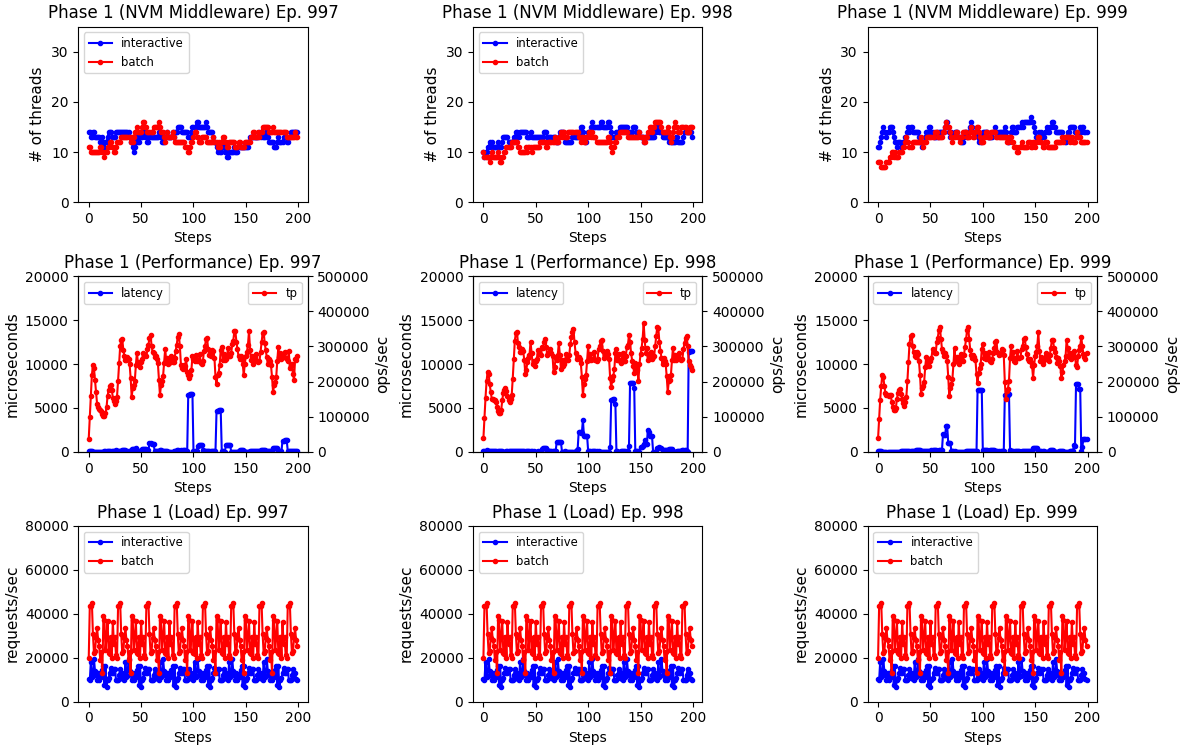
\includegraphics[width=\textwidth,height=\textheight,keepaspectratio,angle=0]{images/rl_training_phase1.png}
    \caption{Learned Pattern Phase 1}
    \label{fig:learned_phase_1}
  \end{figure}

  \begin{figure}[ht]
    \centering
    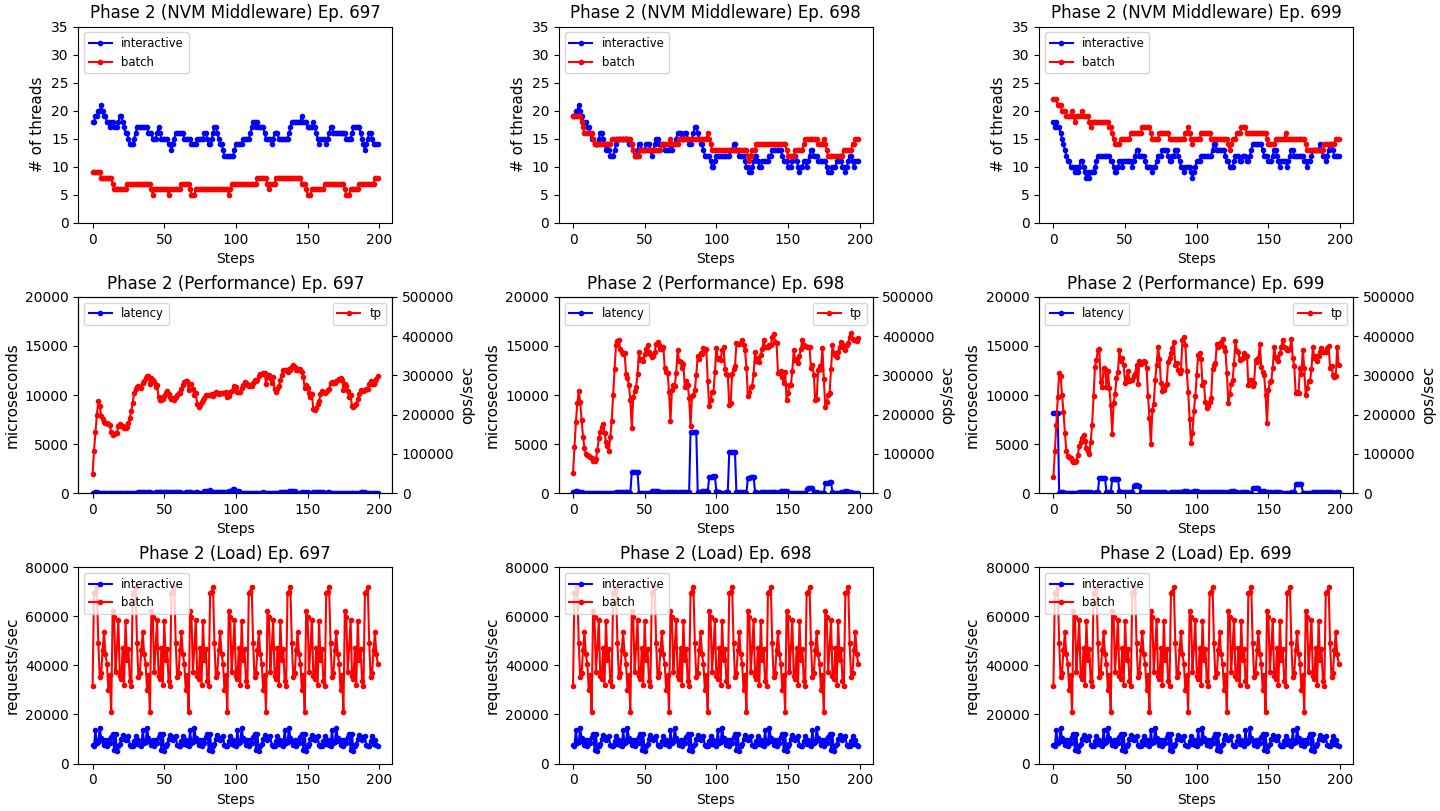
\includegraphics[width=\textwidth,height=\textheight,keepaspectratio,angle=0]{images/rl_training_phase2.png}
    \caption{Learned Pattern Phase 2}
    \label{fig:learned_phase_2}
  \end{figure}

  \begin{figure}[ht]
    \centering
    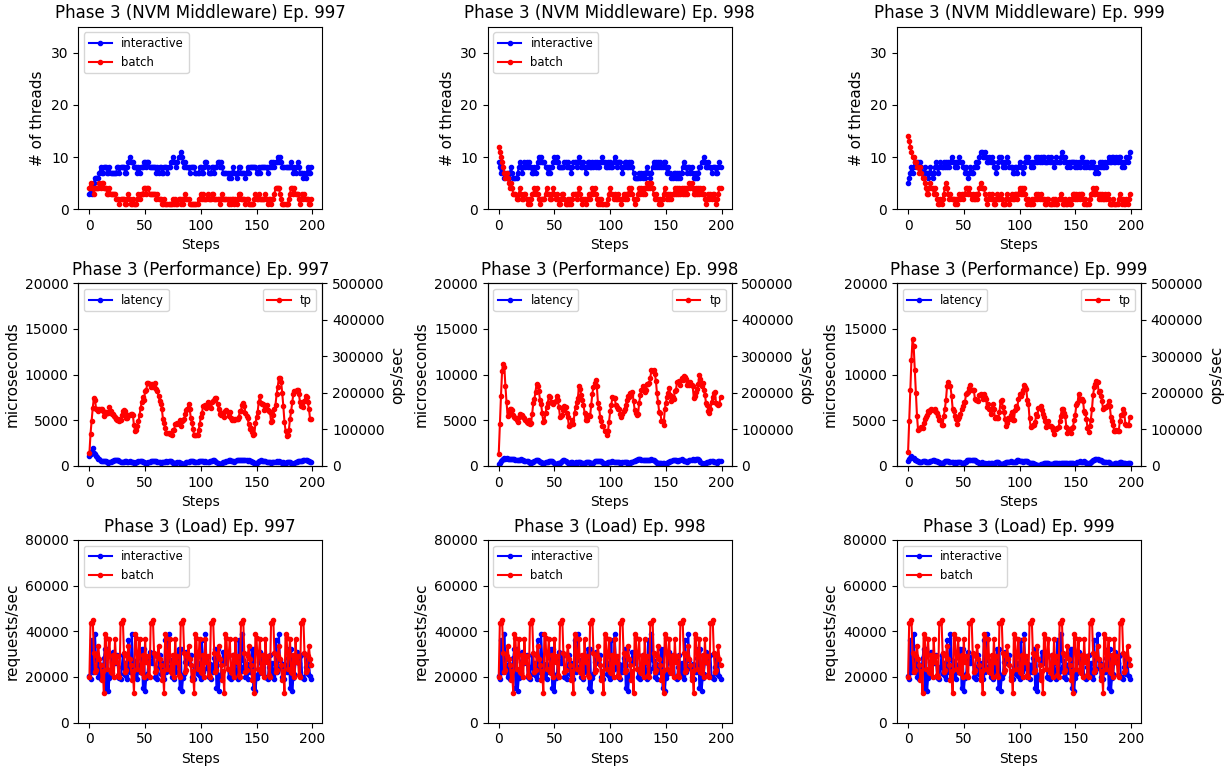
\includegraphics[width=\textwidth,height=\textheight,keepaspectratio,angle=0]{images/rl_training_phase3.png}
    \caption{Learned Pattern Phase 3}
    \label{fig:learned_phase_3}
  \end{figure}

  \begin{figure}[ht]
    \centering
    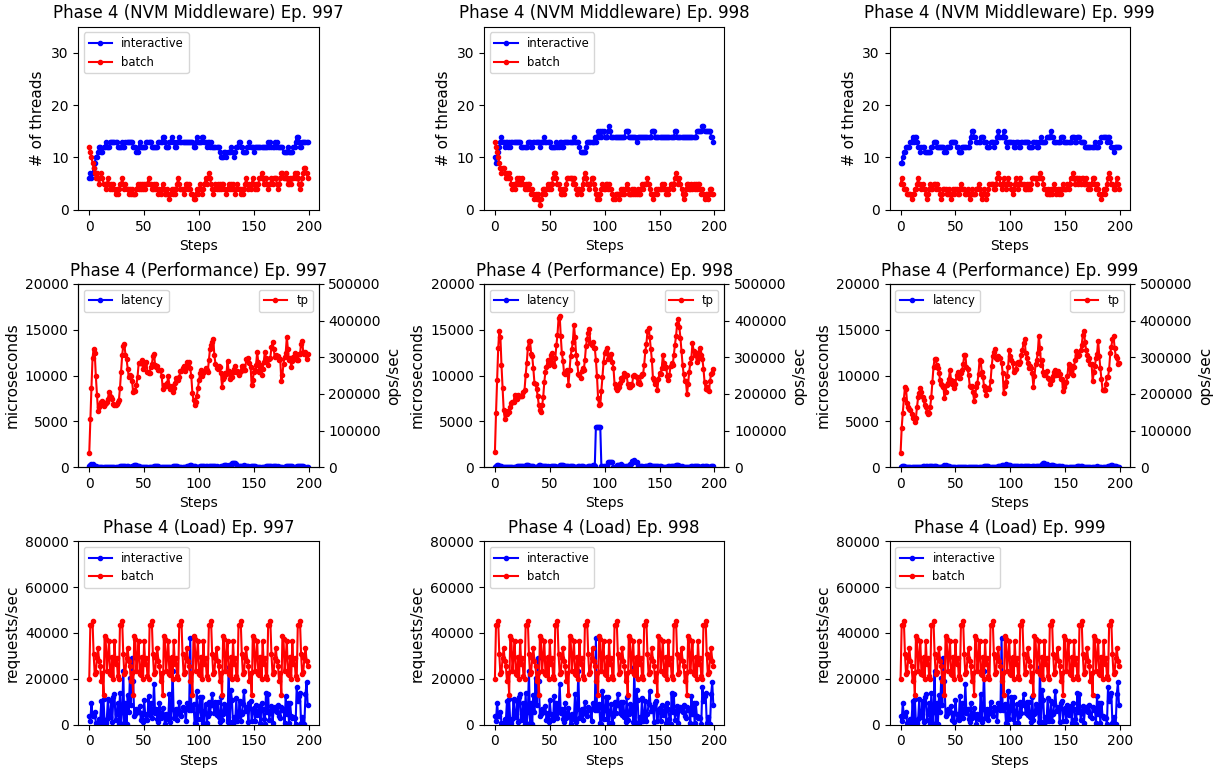
\includegraphics[width=\textwidth,height=\textheight,keepaspectratio,angle=0]{images/rl_training_phase4.png}
    \caption{Learned Pattern Phase 4}
    \label{fig:learned_phase_4}
  \end{figure}